\documentclass{article}

% if you need to pass options to natbib, use, e.g.:
%     \PassOptionsToPackage{numbers, compress}{natbib}
% before loading neurips_2018

% ready for submission
% \usepackage{neurips_2018}

% to compile a preprint version, e.g., for submission to arXiv, add add the
% [preprint] option:
%     \usepackage[preprint]{neurips_2018}

% to compile a camera-ready version, add the [final] option, e.g.:
     \usepackage[final]{neurips_2018}

% to avoid loading the natbib package, add option nonatbib:
%     \usepackage[nonatbib]{neurips_2018}

\usepackage[utf8]{inputenc} % allow utf-8 input
\usepackage[T1]{fontenc}    % use 8-bit T1 fonts
\usepackage{hyperref}       % hyperlinks
\usepackage{url}            % simple URL typesetting
\usepackage{booktabs}       % professional-quality tables
\usepackage{amsfonts}       % blackboard math symbols
\usepackage{nicefrac}       % compact symbols for 1/2, etc.
\usepackage{microtype}      % microtypography

\usepackage{tabularx} % For tables with specified width
\usepackage{hyperref} % For hyperlinks
\usepackage{booktabs} % For better table lines
\usepackage{graphicx} % For including images
\usepackage{subcaption} % For subfigures

\title{Predicting Cell Types in Non-Human Single Cell RNA Sequencing Data}

% The \author macro works with any number of authors. There are two commands
% used to separate the names and addresses of multiple authors: \And and \AND.
%
% Using \And between authors leaves it to LaTeX to determine where to break the
% lines. Using \AND forces a line break at that point. So, if LaTeX puts 3 of 4
% authors names on the first line, and the last on the second line, try using
% \AND instead of \And before the third author name.

\author{
  Sean Connelly \\
  % examples of more authors
  \And
  Ryan Videgar-Laird \\
  \AND
  Stephanie Ting \\
}

\begin{document}
% \nipsfinalcopy is no longer used

\maketitle

\section{Introduction}

NeurIPS requires electronic submissions.  The electronic submission site is
\begin{center}
  \url{https://cmt.research.microsoft.com/NeurIPS2018/}
\end{center}

Please read the instructions below carefully and follow them faithfully.

\subsection{Style}

Papers to be submitted to NeurIPS 2018 must be prepared according to the
instructions presented here. Papers may only be up to eight pages long,
including figures. Additional pages \emph{containing only acknowledgments and/or
  cited references} are allowed. Papers that exceed eight pages of content
(ignoring references) will not be reviewed, or in any other way considered for
presentation at the conference.

The margins in 2018 are the same as since 2007, which allow for $\sim$$15\%$
more words in the paper compared to earlier years.

Authors are required to use the NeurIPS \LaTeX{} style files obtainable at the
NeurIPS website as indicated below. Please make sure you use the current files
and not previous versions. Tweaking the style files may be grounds for
rejection.

\subsection{Retrieval of style files}

The style files for NeurIPS and other conference information are available on
the World Wide Web at
\begin{center}
  \url{http://www.neurips.cc/}
\end{center}
The file \verb+neurips_2018.pdf+ contains these instructions and illustrates the
various formatting requirements your NeurIPS paper must satisfy.

The only supported style file for NeurIPS 2018 is \verb+neurips_2018.sty+,
rewritten for \LaTeXe{}.  \textbf{Previous style files for \LaTeX{} 2.09,
  Microsoft Word, and RTF are no longer supported!}

The \LaTeX{} style file contains three optional arguments: \verb+final+, which
creates a camera-ready copy, \verb+preprint+, which creates a preprint for
submission to, e.g., arXiv, and \verb+nonatbib+, which will not load the
\verb+natbib+ package for you in case of package clash.

\paragraph{New preprint option for 2018}
If you wish to post a preprint of your work online, e.g., on arXiv, using the
NeurIPS style, please use the \verb+preprint+ option. This will create a
nonanonymized version of your work with the text ``Preprint. Work in progress.''
in the footer. This version may be distributed as you see fit. Please \textbf{do
  not} use the \verb+final+ option, which should \textbf{only} be used for
papers accepted to NeurIPS.

At submission time, please omit the \verb+final+ and \verb+preprint+
options. This will anonymize your submission and add line numbers to aid
review. Please do \emph{not} refer to these line numbers in your paper as they
will be removed during generation of camera-ready copies.

The file \verb+neurips_2018.tex+ may be used as a ``shell'' for writing your
paper. All you have to do is replace the author, title, abstract, and text of
the paper with your own.

The formatting instructions contained in these style files are summarized in
Sections \ref{gen_inst}, \ref{headings}, and \ref{others} below.

\section{Related Work}
\label{gen_inst}

The text must be confined within a rectangle 5.5~inches (33~picas) wide and
9~inches (54~picas) long. The left margin is 1.5~inch (9~picas).  Use 10~point
type with a vertical spacing (leading) of 11~points.  Times New Roman is the
preferred typeface throughout, and will be selected for you by default.
Paragraphs are separated by \nicefrac{1}{2}~line space (5.5 points), with no
indentation.

The paper title should be 17~point, initial caps/lower case, bold, centered
between two horizontal rules. The top rule should be 4~points thick and the
bottom rule should be 1~point thick. Allow \nicefrac{1}{4}~inch space above and
below the title to rules. All pages should start at 1~inch (6~picas) from the
top of the page.

For the final version, authors' names are set in boldface, and each name is
centered above the corresponding address. The lead author's name is to be listed
first (left-most), and the co-authors' names (if different address) are set to
follow. If there is only one co-author, list both author and co-author side by
side.

Please pay special attention to the instructions in Section \ref{others}
regarding figures, tables, acknowledgments, and references.

\section{Methods}
\label{headings}

All headings should be lower case (except for first word and proper nouns),
flush left, and bold.

First-level headings should be in 12-point type.

\subsection{Headings: second level}

Second-level headings should be in 10-point type.

\subsubsection{Headings: third level}

Third-level headings should be in 10-point type.

\paragraph{Paragraphs}

There is also a \verb+\paragraph+ command available, which sets the heading in
bold, flush left, and inline with the text, with the heading followed by 1\,em
of space.

\section{Preliminary Results}
\label{others}

\begin{table}[h]
  \caption{Summary of datasets that will be used in this study.}
  \label{tab:summary}
  \centering
  \begin{tabularx}{\textwidth}{lXll}
    \toprule
    \textbf{Host} & \textbf{Source} & \textbf{Reference} & \textbf{Cells} \\
    \midrule
    Parasite & \href{https://github.com/vhowick/MalariaCellAtlas/tree/master/Expression_Matrices/10X/pf10xIDC}{GitHub} & Howick et al. 2019 & 6,737 \\
    \midrule
    Parasite & GSE146737 & Wendt et al. 2020 & 43,642 \\
    \midrule
    Parasite & \href{https://zenodo.org/record/5163554\#.YQvu2ZNKjUo}{Zenodo} & Briggs et al. 2021 & 8,599 \\
    \midrule
    Parasite & \href{https://github.com/umbibio/scBabesiaAtlases}{GitHub} & Rezvani et al. 2022 & 8,719-12,910 \\
    \midrule
    Human & TENxPBMCData R package (Kasper et al. 2021) & 10X Genomics & 3,000 \\
    \midrule
    Human & scRNAseq package (Risso and Cole, 2021) & Lawlor et al. 2017 & 978 \\
    \midrule
    Human & GSE151530 & Ma et al. 2021 and Ma et al. 2022 & 56,721 \\
    \midrule
    Mouse & scRNAseq package (Risso and Cole, 2021) & Zeisel et al. 2015 & 3,005 \\
    \midrule
    Zebrafish & GSE106587 & Farrell et al. 2018 & 38,731 \\
    \midrule
    Non-human primate & GSE156755 & Speranza et al. 2021 & 100,795 \\
    \bottomrule
  \end{tabularx}
\end{table}

\begin{figure}
  \centering
  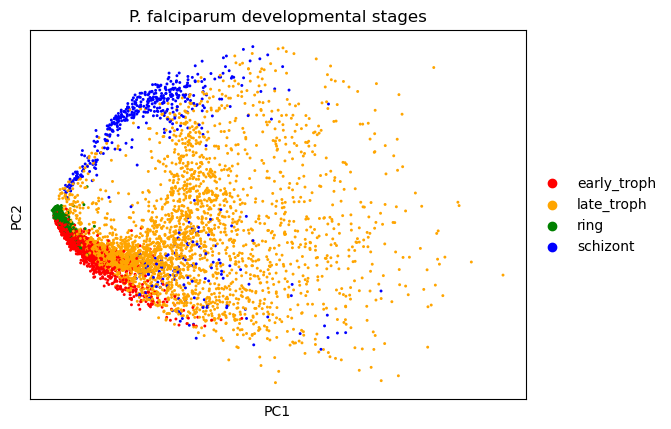
\includegraphics[width=0.8\textwidth]{figures/pca_Pf.png}
  \caption{Principal components analysis of \textit{P. falciparum} single cell RNA sequencing data, colored by lifecycle stage.}
\end{figure}

\begin{figure}[htbp]
  \centering
  
  \begin{subfigure}[b]{0.3\textwidth}
      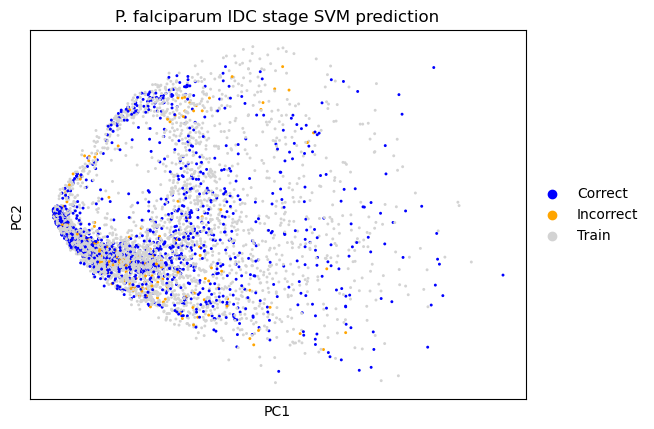
\includegraphics[width=\textwidth]{figures/pca_Pf_prediction_SVM.png}
      \caption{PCA of predictions from SVM model.}
      \label{fig:sub1}
  \end{subfigure}
  \hfill
  \begin{subfigure}[b]{0.3\textwidth}
      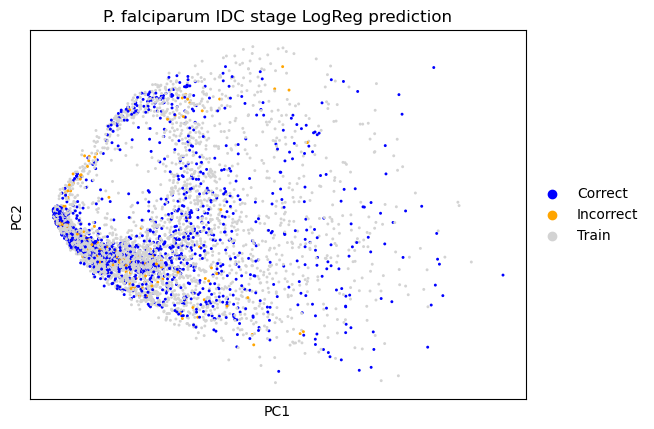
\includegraphics[width=\textwidth]{figures/pca_Pf_prediction_LogReg.png}
      \caption{PCA of predictions from logistic regression model.}
      \label{fig:sub2}
  \end{subfigure}
  \hfill
  \begin{subfigure}[b]{0.3\textwidth}
      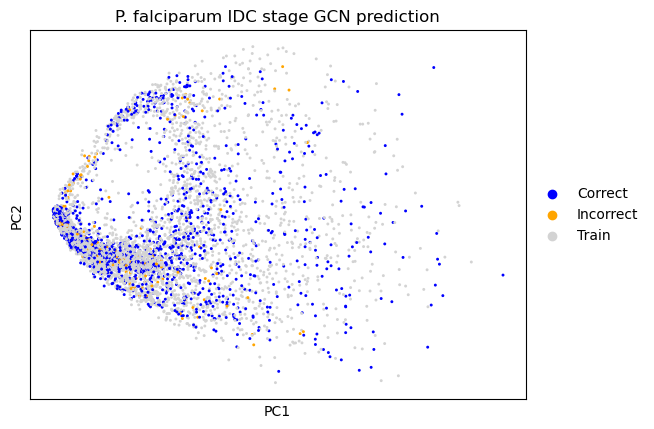
\includegraphics[width=\textwidth]{figures/pca_Pf_prediction_GCN.png}
      \caption{PCA of predictions from graph convolutional network model.}
      \label{fig:sub3}
  \end{subfigure}
  
  \caption{Model performance visualized on PCA plots.}
  \label{fig:main}
\end{figure}

\begin{figure}
  \centering
  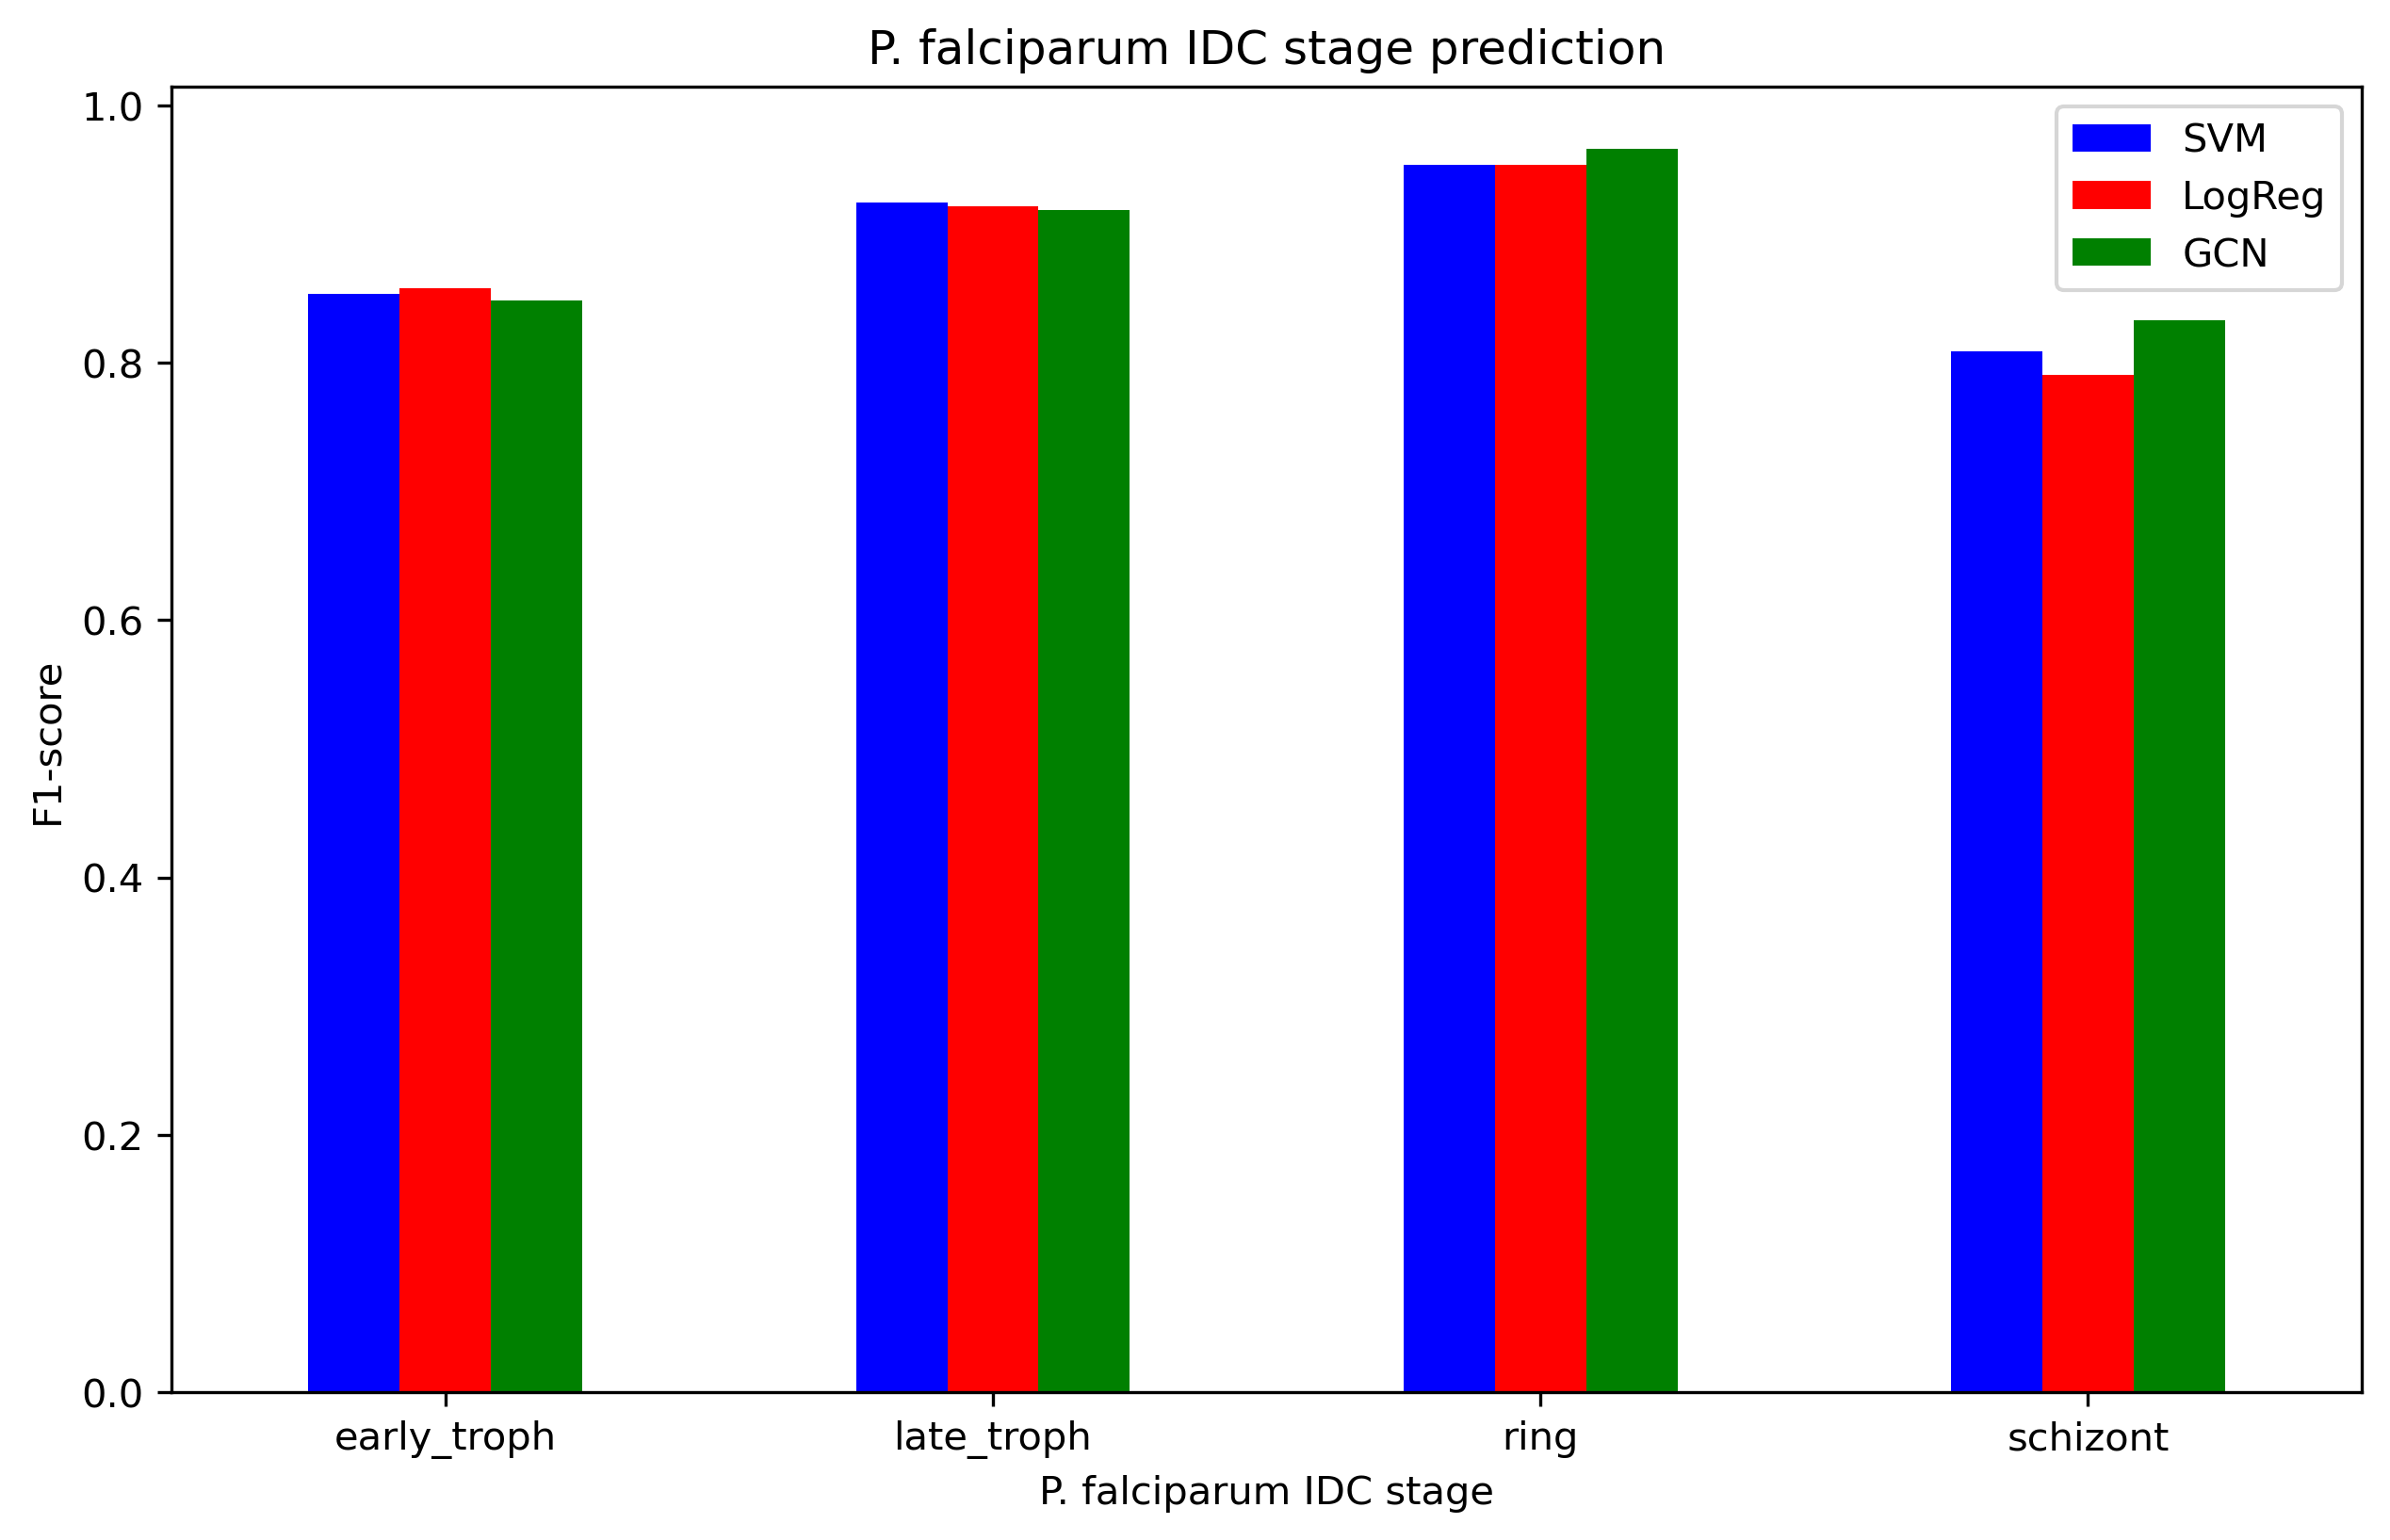
\includegraphics[width=0.8\textwidth]{figures/Pf_prediction.png}
  \caption{Prediction accuracy of models on \textit{P. falciparum} single cell RNA sequencing data.}
\end{figure}

These instructions apply to everyone.

\subsection{Citations within the text}

The \verb+natbib+ package will be loaded for you by default.  Citations may be
author/year or numeric, as long as you maintain internal consistency.  As to the
format of the references themselves, any style is acceptable as long as it is
used consistently.

The documentation for \verb+natbib+ may be found at
\begin{center}
  \url{http://mirrors.ctan.org/macros/latex/contrib/natbib/natnotes.pdf}
\end{center}
Of note is the command \verb+\citet+, which produces citations appropriate for
use in inline text.  For example,
\begin{verbatim}
   \citet{hasselmo} investigated\dots
\end{verbatim}
produces
\begin{quote}
  Hasselmo, et al.\ (1995) investigated\dots
\end{quote}

If you wish to load the \verb+natbib+ package with options, you may add the
following before loading the \verb+neurips_2018+ package:
\begin{verbatim}
   \PassOptionsToPackage{options}{natbib}
\end{verbatim}

If \verb+natbib+ clashes with another package you load, you can add the optional
argument \verb+nonatbib+ when loading the style file:
\begin{verbatim}
   \usepackage[nonatbib]{neurips_2018}
\end{verbatim}

As submission is double blind, refer to your own published work in the third
person. That is, use ``In the previous work of Jones et al.\ [4],'' not ``In our
previous work [4].'' If you cite your other papers that are not widely available
(e.g., a journal paper under review), use anonymous author names in the
citation, e.g., an author of the form ``A.\ Anonymous.''

\subsection{Footnotes}

Footnotes should be used sparingly.  If you do require a footnote, indicate
footnotes with a number\footnote{Sample of the first footnote.} in the
text. Place the footnotes at the bottom of the page on which they appear.
Precede the footnote with a horizontal rule of 2~inches (12~picas).

Note that footnotes are properly typeset \emph{after} punctuation
marks.\footnote{As in this example.}

\subsection{Figures}

\begin{figure}
  \centering
  \fbox{\rule[-.5cm]{0cm}{4cm} \rule[-.5cm]{4cm}{0cm}}
\end{figure}

All artwork must be neat, clean, and legible. Lines should be dark enough for
purposes of reproduction. The figure number and caption always appear after the
figure. Place one line space before the figure caption and one line space after
the figure. The figure caption should be lower case (except for first word and
proper nouns); figures are numbered consecutively.

You may use color figures.  However, it is best for the figure captions and the
paper body to be legible if the paper is printed in either black/white or in
color.

\subsection{Tables}

All tables must be centered, neat, clean and legible.  The table number and
title always appear before the table.  See Table~\ref{sample-table}.

Place one line space before the table title, one line space after the
table title, and one line space after the table. The table title must
be lower case (except for first word and proper nouns); tables are
numbered consecutively.

Note that publication-quality tables \emph{do not contain vertical rules.} We
strongly suggest the use of the \verb+booktabs+ package, which allows for
typesetting high-quality, professional tables:
\begin{center}
  \url{https://www.ctan.org/pkg/booktabs}
\end{center}
This package was used to typeset Table~\ref{sample-table}.

\begin{table}
  \caption{Sample table title}
  \label{sample-table}
  \centering
  \begin{tabular}{lll}
    \toprule
    \multicolumn{2}{c}{Part}                   \\
    \cmidrule(r){1-2}
    Name     & Description     & Size ($\mu$m) \\
    \midrule
    Dendrite & Input terminal  & $\sim$100     \\
    Axon     & Output terminal & $\sim$10      \\
    Soma     & Cell body       & up to $10^6$  \\
    \bottomrule
  \end{tabular}
\end{table}

\section{Future Plans}

Please prepare submission files with paper size ``US Letter,'' and not, for
example, ``A4.''

Fonts were the main cause of problems in the past years. Your PDF file must only
contain Type 1 or Embedded TrueType fonts. Here are a few instructions to
achieve this.

\begin{itemize}

\item You should directly generate PDF files using \verb+pdflatex+.

\item You can check which fonts a PDF files uses.  In Acrobat Reader, select the
  menu Files$>$Document Properties$>$Fonts and select Show All Fonts. You can
  also use the program \verb+pdffonts+ which comes with \verb+xpdf+ and is
  available out-of-the-box on most Linux machines.

\item The IEEE has recommendations for generating PDF files whose fonts are also
  acceptable for NeurIPS. Please see
  \url{http://www.emfield.org/icuwb2010/downloads/IEEE-PDF-SpecV32.pdf}

\item \verb+xfig+ "patterned" shapes are implemented with bitmap fonts.  Use
  "solid" shapes instead.

\item The \verb+\bbold+ package almost always uses bitmap fonts.  You should use
  the equivalent AMS Fonts:
\begin{verbatim}
   \usepackage{amsfonts}
\end{verbatim}
followed by, e.g., \verb+\mathbb{R}+, \verb+\mathbb{N}+, or \verb+\mathbb{C}+
for $\mathbb{R}$, $\mathbb{N}$ or $\mathbb{C}$.  You can also use the following
workaround for reals, natural and complex:
\begin{verbatim}
   \newcommand{\RR}{I\!\!R} %real numbers
   \newcommand{\Nat}{I\!\!N} %natural numbers
   \newcommand{\CC}{I\!\!\!\!C} %complex numbers
\end{verbatim}
Note that \verb+amsfonts+ is automatically loaded by the \verb+amssymb+ package.

\end{itemize}

If your file contains type 3 fonts or non embedded TrueType fonts, we will ask
you to fix it.

\subsection{Margins in \LaTeX{}}

Most of the margin problems come from figures positioned by hand using
\verb+\special+ or other commands. We suggest using the command
\verb+\includegraphics+ from the \verb+graphicx+ package. Always specify the
figure width as a multiple of the line width as in the example below:
\begin{verbatim}
   \usepackage[pdftex]{graphicx} ...
   \includegraphics[width=0.8\linewidth]{myfile.pdf}
\end{verbatim}
See Section 4.4 in the graphics bundle documentation
(\url{http://mirrors.ctan.org/macros/latex/required/graphics/grfguide.pdf})

A number of width problems arise when \LaTeX{} cannot properly hyphenate a
line. Please give LaTeX hyphenation hints using the \verb+\-+ command when
necessary.

\subsubsection*{Acknowledgments}

Use unnumbered third level headings for the acknowledgments. All acknowledgments
go at the end of the paper. Do not include acknowledgments in the anonymized
submission, only in the final paper.

\section*{References}

References follow the acknowledgments. Use unnumbered first-level heading for
the references. Any choice of citation style is acceptable as long as you are
consistent. It is permissible to reduce the font size to \verb+small+ (9 point)
when listing the references. {\bf Remember that you can use more than eight
  pages as long as the additional pages contain \emph{only} cited references.}
\medskip

\small

\begin{enumerate}
  \item Heumos, L., et al. (2023). Best practices for single-cell analysis across modalities. \textit{Nat Rev Genet}, 24, 550–572.
  \item Yang, F., et al. (2022). scBERT as a large-scale pretrained deep language model for cell type annotation of single-cell RNA-seq data. \textit{Nat Mach Intell}, 4, 852–866.
  \item Chen, J., et al. (2023). Transformer for one stop interpretable cell type annotation. \textit{Nat Commun}, 14, 223.
  \item Howick, V. M., et al. (2019). The Malaria Cell Atlas: Single parasite transcriptomes across the complete \textit{Plasmodium} life cycle. \textit{Science}, 365, eaaw2619.
  \item Kipf, T. N., \& Welling, M. (2016). Semi-Supervised Classification with Graph Convolutional Networks. arXiv:1609.02907.
  \item Pedregosa, F., et al. (2012). Scikit-learn: Machine Learning in Python. \textit{J Mach Learn Res}, 12, 2825–30.
  \item Spektral. \url{https://github.com/danielegrattarola/spektral}
  \item F1 Score. \url{https://towardsdatascience.com/the-f1-score-bec2bbc38aa6}
  \item TENxPBMCData. \url{https://bioconductor.org/packages/release/data/experiment/html/TENxPBMCData.html}
  \item scRNAseq. \url{https://bioconductor.org/packages/release/data/experiment/manuals/scRNAseq/man/scRNAseq.pdf}
  \item Lawlor, N., et al. (2017). Single-cell transcriptomes identify human islet cell signatures and reveal cell-type-specific expression changes in type 2 diabetes. \textit{Genome Res}, 27(2), 208-222.
  \item Zeisel, A., et al. (2015). Cell types in the mouse cortex and hippocampus revealed by single-cell RNA-seq. \textit{Science}, 347, 1138-1142.
  \item Ma, L., et al. (2021). Single-cell atlas of tumor cell evolution in response to therapy in hepatocellular carcinoma and intrahepatic cholangiocarcinoma. \textit{J Hepatol}, 75(6), 1397-1408.
  \item Ma, L., et al. (2022). Multiregional single-cell dissection of tumor and immune cells reveals stable lock-and-key features in liver cancer. \textit{Nat Commun}, 13(1), 7533.
  \item Farrell, J. A., et al. (2018). Single-cell reconstruction of developmental trajectories during zebrafish embryogenesis. \textit{Science}, 360(6392).
  \item Speranza, E., et al. (2021). Single-cell RNA sequencing reveals SARS-CoV-2 infection dynamics in lungs of African green monkeys. \textit{Sci Transl Med}, 13(578).
  \item Wendt, G., et al. (2020). A single-cell RNA-seq atlas of Schistosoma mansoni identifies a key regulator of blood feeding. \textit{Science}, 369(6511), 1644-1649.
  \item Briggs, E. M., et al. (2021). Single-cell transcriptomic analysis of bloodstream Trypanosoma brucei reconstructs cell cycle progression and developmental quorum sensing. \textit{Nat Commun}, 12, 5268.
  \item Rezvani, Y., et al. (2022). Comparative single-cell transcriptional atlases of Babesia species reveal conserved and species-specific expression profiles. \textit{PLOS Biol}, 20(9), e3001816.
  \end{enumerate}
\end{document}
